% ~ 1 page
% !TeX root = ./main.tex

\section{Empirical Study}
\label{sec:experiments}
We seek to answer the following six research questions (RQs) through our experimental evaluations.
\begin{itemize}
    \item\underline{\textbf{RQ1}}: How accurate is the QoS model developed in~\pref{sec:system_model} compared to others in the literature?
    \item\underline{\textbf{RQ2}}: How do different EMO frameworks compare on the VNFPP?
    \item\underline{\textbf{RQ3}}: Is an accurate QoS model beneficial compared to surrogate models used in the literature?
    \item\underline{\textbf{RQ4}}: Does the proposed solution representation improve upon alternative solution representations?
    \item\underline{\textbf{RQ5}}: How does the tailored EMO algorithm compare against the state-of-the-art peers?
    \item\underline{\textbf{RQ6}}: How well do the proposed operators cope with challenging constraints in VNFPP?
\end{itemize}

%\begin{table}[t]
%    \vspace{1em}
%    \centering
%    
%    \caption{Parameter settings used in evaluation}
%    \label{tab:parameter}
%    \begin{tabular}{ll}
%        \toprule
%        Parameter                             & Setting        \\
%        \midrule
%        Mean service arrival rate             & 10 requests/ms \\
%        Variance service arrival rate         & 3 requests/ms  \\
%        \midrule
%        Per port service rate                 & 20 requests/ms \\
%        Per port queue length                 & 20 requests    \\
%        Server active energy cost             & 30 kw/h        \\
%        Server idle energy cost               & 10 kw/h        \\
%        \midrule
%        Min. data center utilization          & 60\%           \\
%        Mean service length                   & 5 VNFs         \\
%        Variance service length               & 1 VNFs         \\
%        Min service length                    & 2 VNFs         \\
%        \midrule
%        Mean VNF service rate                 & 10 requests/ms \\
%        Variance VNF service rate             & 3 requests/ms  \\
%        VNF queue length                      & 20             \\
%        \midrule
%        Model tolerance $\left(\delta\right)$ & 5.0            \\
%        Min. iterations $\left(\gamma\right)$ & 10             \\
%        \midrule
%        Population size $\left(n\right)$      & 120            \\
%        Mutation rate                         & 1/$n$          \\
%        Crossover probability                 & 0.9            \\
%        Number of evaluations                 & 1200           \\
%        \bottomrule
%    \end{tabular}
%\end{table}

\subsection{Parameter settings}
The parameter settings used in this work are listed in Table II in the Appendix D. To reflect the mechanism of real switches, the service rate and queue length of each switch in our model are the sum of the service rates and queue lengths of each port. For example, a switch with $8$ ports will have a service rate of $8\times 20=160$ requests/ms. To create a VNFPP instance, we generate enough services to hit the target minimum data center utilization. For example, if the data center has $1,000$ VMs, the expected service length is $5$ and the target data center utilization is $50$\%, then there will be $100$ distinct services. Next, the service arrival rate and length and the VNF service rate are set for each service and VNF by sampling from a Gaussian distribution with the means and variances specified in Table II in the Appendix D.

\subsection{Evaluation of QoS Model Accuracy}
\label{sec:model_accuracy}

\subsubsection{Methods}
The QoS model developed in~\pref{sec:system_model} stands for the foundation of this study. Its correctness and accuracy determine whether our algorithm is applicable to real-world problems. To answer RQ1, we evaluate the accuracy of the model by comparing its predictions against benchmark measurements taken from a simulated data center.

\textcolor{red}{To create the benchmark, we generate $100$ VNFPP problems for a data center with $412$ servers to constitute a diverse set of problems. Then, we use our proposed initialization operator (see \pref{sec:operators}) to generate $100$ candidate solutions for each problem.} Next, we evaluate each solution by using our proposed model and select four solutions for evaluation: 1) the one with the lowest latency; 2) the one with the lowest packet loss; 3) the one with the lowest energy consumption; and 4) the one that best balances all objectives. By using diverse solutions, we can rule out any inaccuracy reflected by the model. For example, if the model is poor at predicting the latency, the data set will contain a solution with a high expected latency that highlights this issue. %As simulation is slow we are only able to evaluate a select number of solutions. 

To get accurate measurements for the benchmark, we apply a discrete event simulator (DES) to calculate each metric of a solution. A DES simulates the transmission of each packet through the data center to produce accurate measurements of the QoS and energy consumption. In our experiments, the DES is based on the same assumptions introduced in \pref{sec:system_model} and it is used to evaluate each solution for a range of arrival rates.

We compare our model against two other accurate models used in the literature.%: an M/M/1 queueing model and an M/M/1/B$_c$ queueing model.
\begin{itemize}
    \item \underline{M/M/1 queueing model}: As one of most popular models in the literature~\cite{PeiHXLWW20,JemaaPP16,BaumgartnerRB15}, it models the data center as a network of queues and assumes that each queue has an infinite length. Under this assumption, there is no packet loss. However, if the arrival rate at a queue is greater than or equal to its service rate, the length of the queue will tend towards infinity that leads the waiting time to approach infinity and the utilization to approach $100$\%.
    \item \underline{M/M/1/B$_c$ queuing model}: In contrast, this model consider queues with a finite length. Existing M/M/1/B$_c$ queueing models like~\cite{ChuaWZSH16} consider packet loss but not feedback loops. In essence, they calculate the instantaneous arrival rate and packet loss at each data center component when the services are first started.
\end{itemize}

\subsubsection{Results}
\pref{fig:model_sim} shows the estimates of each metric by different models benchmarked against the ground-truth measurements. The closer the model matches the benchmark, the more accurate the model is. From the results, we find that our proposed model is significantly more accurate than the other peer queueing models. This reflects how our model correctly captures the impact of feedback loops on the QoS and energy consumption.

In contrast, the M/M/1/B$_c$ queueing model, which does not account for feedback loops, is overly pessimistic with a high latency, packet loss and energy consumption. This is because the M/M/1/B$_c$ model calculates the instantaneous arrival rate at the start of operation. As shown in Lemma \ref{lemma:arrival_rate}, this is always higher than the arrival rate after convergence.

Likewise, these results also demonstrate the drawbacks of the commonly used M/M/1 model. First, the model falsely assumes that the queue at a component can grow to an infinite length and as a consequence believes that packet loss is zero in all situations. As a result, the model becomes less reliable as the arrival rate increases and packet loss becomes large.

\vspace{0.5em}
\noindent
\framebox{\parbox{\dimexpr\linewidth-2\fboxsep-2\fboxrule}{
        \textbf{\underline{Response to RQ1:}} \textit{Due to an understanding of the impact of feedback loops, our proposed model gives significantly more accurate estimates of the QoS and energy consumption than other models when packet loss is considered.}
    }}

\begin{figure*}[t!]
    \centering
    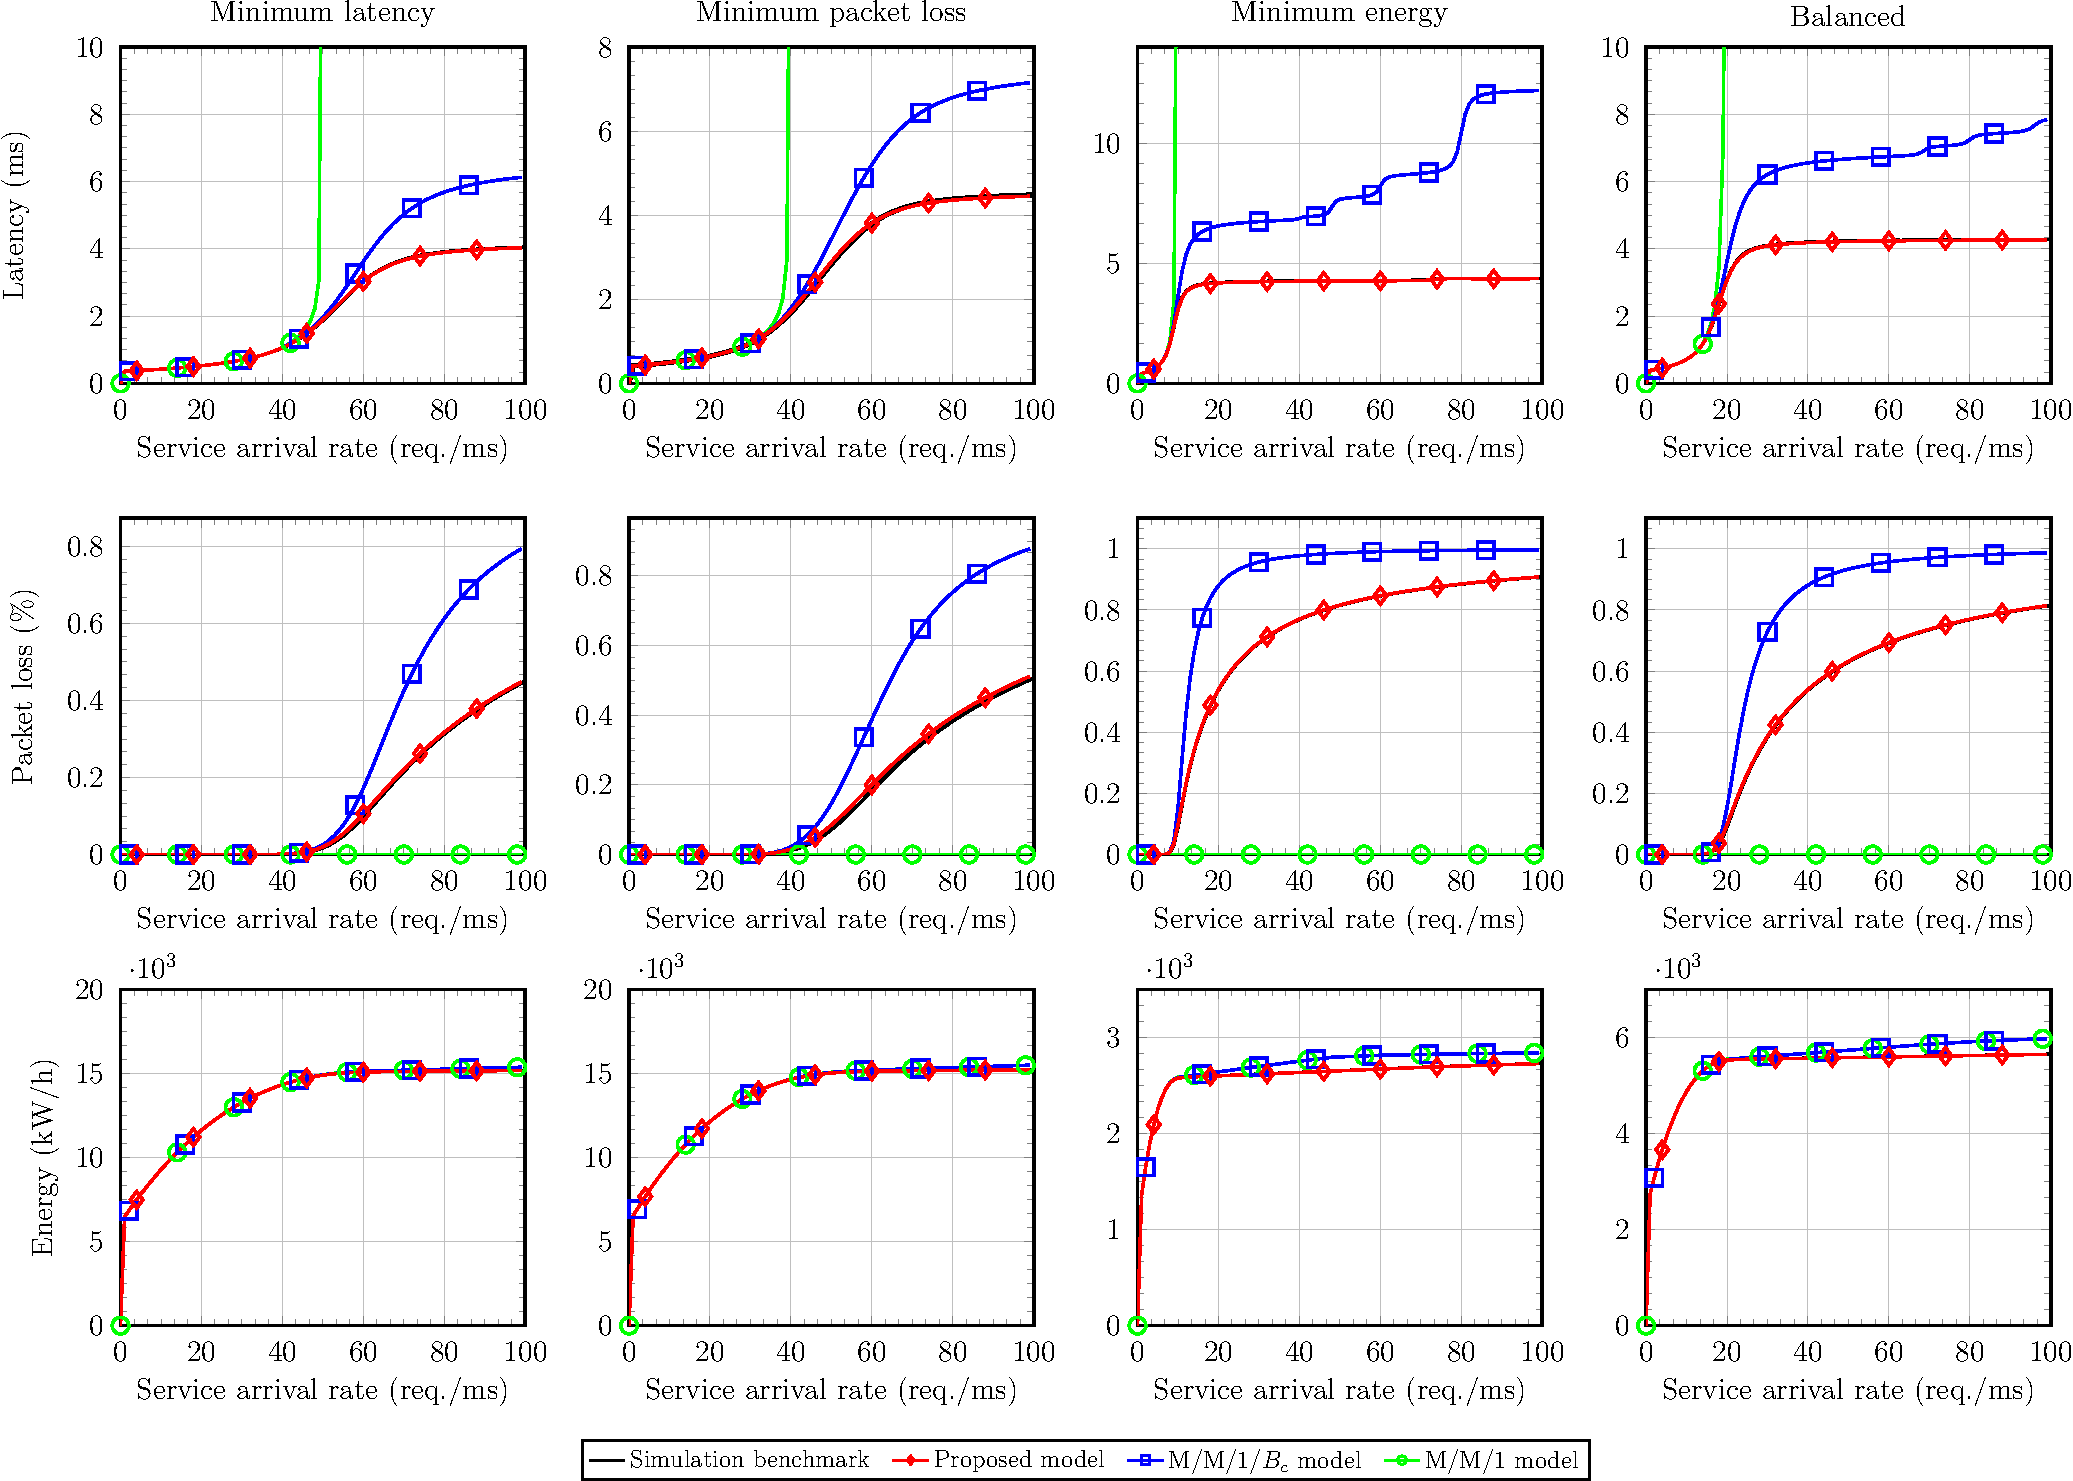
\includegraphics[width=\textwidth]{graphs/general/model_sim-crop}
    \caption{Comparison results of three different metrics estimated by our proposed model against the other two queueing models.}
    \label{fig:model_sim}
\end{figure*}

\subsection{Comparison with Other MOEA Frameworks}
\label{sec:moea_comparison}

\subsubsection{Methods}
\textcolor{red}{To illustrate that our operators can be integrated into any MOEA framework, we compare the quality of solutions obtained when different MOEAs are used with our proposed operators. Specifically, we integrated our proposed operators into three state of the art MOEAs: NSGA-II \cite{DebAPM02}, MOEA/D \cite{ZhangL07} and IBEA \cite{ZitzlerK04}.}

\textcolor{red}{
In our experiments, we generate $30$ VNFPP instances for six data centers with different sizes. To compare the performance of different algorithms, we use the QoS model developed in~\pref{sec:system_model} to evaluate the objective functions of the solutions obtained by different algorithms and use the HV indicator as the performance measure.
}

\textcolor{red}{
\subsubsection{Results}
The results of this test are illustrated in~\pref{fig:moea_comparison}. We found that all algorithm performed similarly, with no algorithm performing consistently significantly better than any other. Given all algorithms performed similarly, we have selected NSGA-II for use in future tests based on its widespread adoption in the literature. 
}

\begin{figure}[t!]
    \centering
    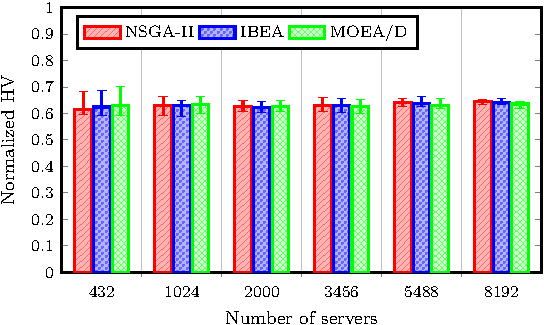
\includegraphics[width=\columnwidth]{graphs/moeas/comparison-crop}
    \caption{Inter-quartile range of the HV for different MOEAs.}
    \label{fig:moea_comparison}
\end{figure}

\vspace{0.5em}
\noindent
\framebox{\parbox{\dimexpr\linewidth-2\fboxsep-2\fboxrule}{
    \textcolor{red}{\textbf{\underline{Response to RQ2:}} \textit{From our empirical results, we find that all MOEAs using our proposed operators performed comparably.}
    }}}

\subsection{Benefit of Queueing Models}
\label{sec:model_benefit}

\subsubsection{Methods}
% \! is to fix the odd space that \cite introduces after the bracket

To answer RQ3, we compare the quality of solutions obtained by our tailored EMO algorithm when using different QoS models including three queueing models studied in~\pref{sec:model_accuracy} and three popular surrogate models briefly introduced as follows.
\begin{itemize}
    % Explain the reasoning behind these surrogates
    \item\underline{Constant waiting time or packet loss (CWTPL)}: As in~\cite{HawiloJS19} and~\cite{VizarretaCMMK17}, this model assumes that the waiting time at each data center component is a constant. In addition, we also keeps the packet loss probability at each component as a constant. Based on these assumptions, we can evaluate the latency and packet loss for each service and apply the metric of the energy consumption developed in~\pref{sec:energy}. All these constitute a three-objective problem that aims to minimize the average latency, packet loss and total energy consumption.

    \item\underline{Resource utilization (RU)}: As in~\cite{ChantreF20,QiSW19} and~\cite{GuoWLQA0Y20}, this model assumes that the waiting time is a function of the CPU demand and the CPU capacity of each VM. In addition, the demand is assumed to determine the packet loss probability as well. Based on these assumptions, we evaluate the latency for each service and apply the metric of the energy consumption developed in~\pref{sec:energy}. All these constitute a two-objective problem that aims to minimize the average latency (and by extension the packet loss) and the total energy consumption.

    \item\underline{Path length and used servers (PLUS)}: This model uses the percentage of used servers to measure the energy consumption (e.g.,~\cite{MiottoLCG19,RankothgeLRL17,LiuZDLGZ18}) and the length of routes for each service as a measure of service latency, packet loss or quality (e.g.,~\cite{LuizelliCBG17,AllegKMA17,BeckB15}). All these constitute a two-objective problem that aims to minimize the path length and the number of used servers.
\end{itemize}

In our experiments, we generate $30$ problem instances of the Fat Tree data center with $432$, $1,024$, $2,000$, $3,456$, $5,488$ and $8,192$ servers respectively. At the end, the non-dominated solutions found by our tailored EMO algorithm with different QoS models are re-evaluated by using the QoS model developed in~\pref{sec:system_model}. The quality of these non-dominated solutions is evaluated by the Hypervolume (HV) indicator~\cite{ZitzlerT99} that measures both the convergence and diversity of the population, simultaneously.

\subsubsection{Results}

From the results shown in Figs.~\ref{fig:model_objectives} and~\ref{fig:model_benefits}, we find that the solutions obtained by using our proposed model and the M/M/1/B$_c$ queueing model are comparable with each other while they are significantly better than those obtained by using other models in terms of the population diversity.

%\pref{fig:model_benefits} shows that the choice of model had a significant impact on the quality and diversity of the solutions in the final population. The populations proposed by our model and the M/M/1/$B_c$ model are more diverse than the alternative models and typically have lower average latency, packet loss and energy consumption. Notably, neither of the models produce significantly better ($p < 0.05$) populations than the other as measured by the HV and a Wilcoxon Rank Sum test \cite{ArcuriB11}. This is despite the M/M/1/$B_c$ model giving less accurate measurements of the metrics. Clearly, strict parity with the simulation is not essential for the algorithm to find good solutions but only that the simulation and model agree on the ordering of solutions, i.e. given any two solutions $x$ and $y$, both models will agree whether $x$ is better, worse or equivalent to $y$ in each objective. From these results and \pref{fig:model_sim}, it seems likely that M/M/1/$B_c$ and our proposed model meet this criteria.

Specifically, populations obtained with the M/M/1 queueing model have poor diversity. This can be attributed to the inability of the M/M/1 queueing model to distinguish solutions by the latency or packet loss metrics. In particular, most solutions obtained by using the M/M/1 queueing model have an infinite latency and no packet loss. This is because if the arrival rate at any data center component is larger than the service rate, the waiting time at that component tends towards infinity. Hence the average latency also tends towards infinity. As all solutions have the same latency and packet loss, the optimization algorithm can only distinguish solutions based on their energy consumption. As a result, only solutions with low energy consumption survive.

For a similar reason, the surrogate models also failed to produce diverse solutions. Despite their differences, none of the surrogate models provide any incentive to vary the number of service instances. For example, both the CWTPL and PLUS models benefit from shorter average routes. However, increasing the number of service instances will also increase the number of servers yet is unlikely to decrease the average service length. Likewise, for the RU model, increasing the number of service instances increases the energy consumption and makes it more difficult for the algorithm to find servers with a low resource utilization.

% \begin{figure*}[t!]
%     \centering

%     \begin{subfigure}[b]{0.24\linewidth}
%         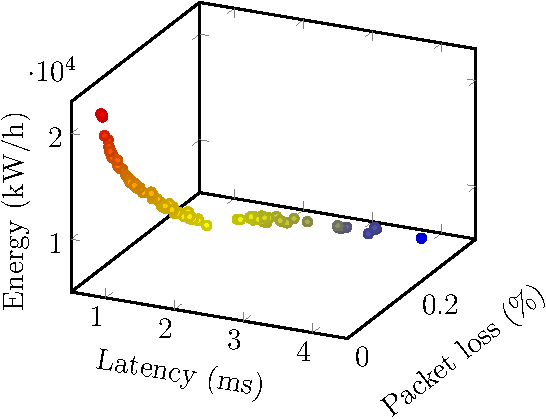
\includegraphics[width=\textwidth]{graphs/model/proposed-crop}
%         \caption{Proposed}
%     \end{subfigure}
%     \begin{subfigure}[b]{0.24\linewidth}
%         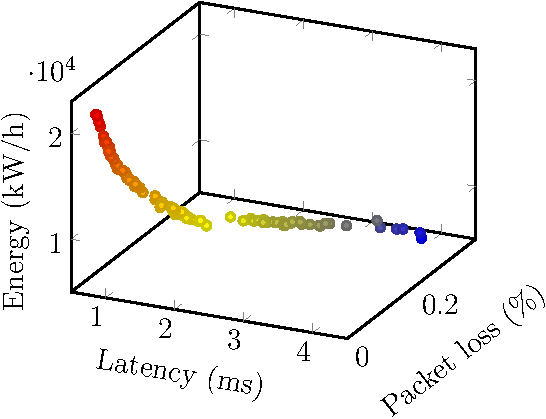
\includegraphics[width=\textwidth]{graphs/model/mm1k-crop}
%         \caption{M/M/1/$B_c$}
%     \end{subfigure}
%     \begin{subfigure}[b]{0.24\linewidth}
%         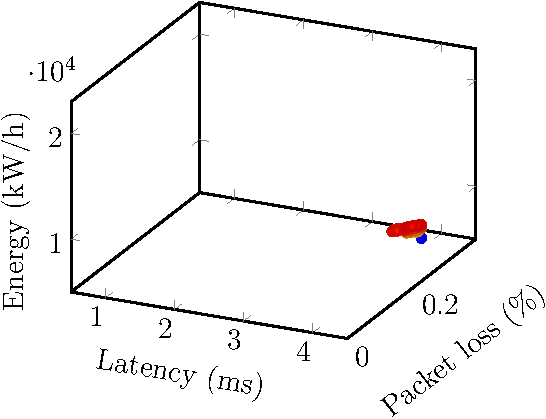
\includegraphics[width=\textwidth]{graphs/model/mm1-crop}
%         \caption{M/M/1}
%     \end{subfigure}
%     \begin{subfigure}[b]{0.24\linewidth}
%         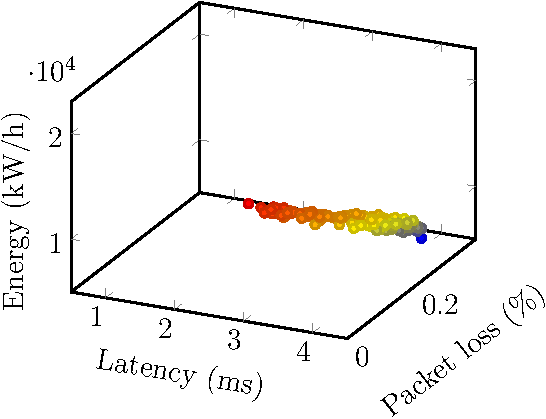
\includegraphics[width=\textwidth]{graphs/model/constant_energy-crop}
%         \caption{CWTPL}
%     \end{subfigure}

%     \vspace{1em}

%     \hspace{7em}
%     \begin{subfigure}[b]{0.24\linewidth}
%         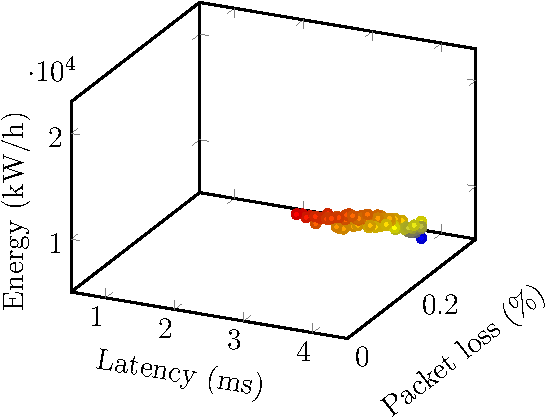
\includegraphics[width=\textwidth]{graphs/model/resources_energy-crop}
%         \caption{RU}
%     \end{subfigure}
%     \hfill
%     \begin{subfigure}[b]{0.24\linewidth}
%         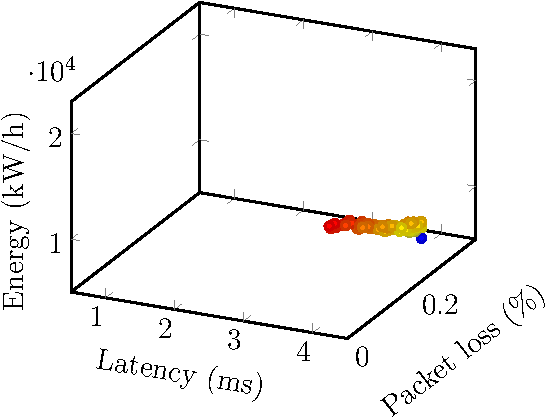
\includegraphics[width=\textwidth]{graphs/model/length_used-crop}
%         \caption{PLUS}
%     \end{subfigure}
%     \hspace{6em}

%     \vspace{1em}
%     \caption{\textcolor{red}{Non-dominated front found by our algorithm when different models are used as the objective function.}}
%     \label{fig:model_objectives}
% \end{figure*}

% \begin{figure*}[t!]
%     \centering

%     \begin{subfigure}[b]{0.16\linewidth}
%         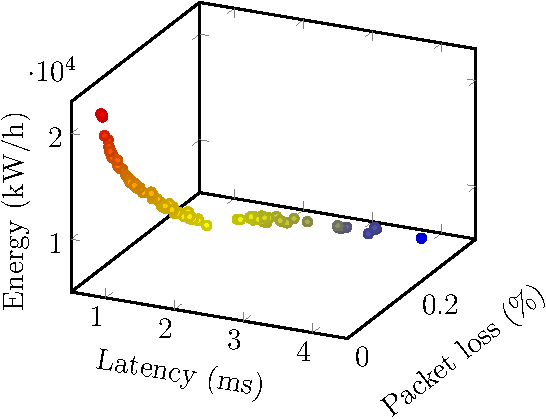
\includegraphics[width=\textwidth]{graphs/model/proposed-crop}
%         \caption{Proposed}
%     \end{subfigure}
%     \begin{subfigure}[b]{0.16\linewidth}
%         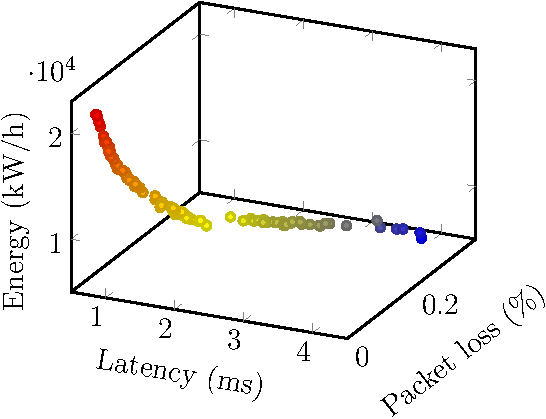
\includegraphics[width=\textwidth]{graphs/model/mm1k-crop}
%         \caption{M/M/1/$B_c$}
%     \end{subfigure}
%     \begin{subfigure}[b]{0.16\linewidth}
%         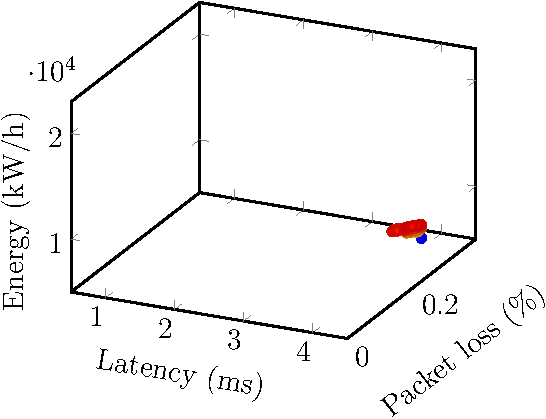
\includegraphics[width=\textwidth]{graphs/model/mm1-crop}
%         \caption{M/M/1}
%     \end{subfigure}
%     \begin{subfigure}[b]{0.16\linewidth}
%         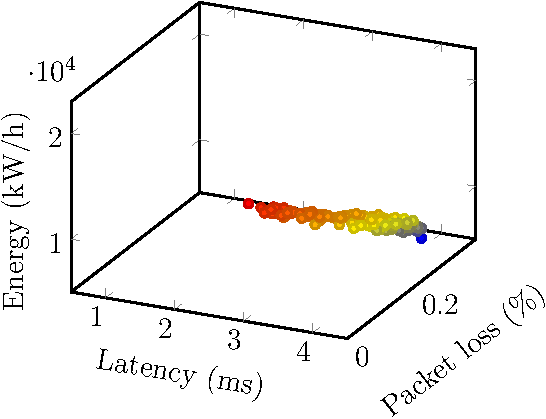
\includegraphics[width=\textwidth]{graphs/model/constant_energy-crop}
%         \caption{CWTPL}
%     \end{subfigure}
%     \begin{subfigure}[b]{0.16\linewidth}
%         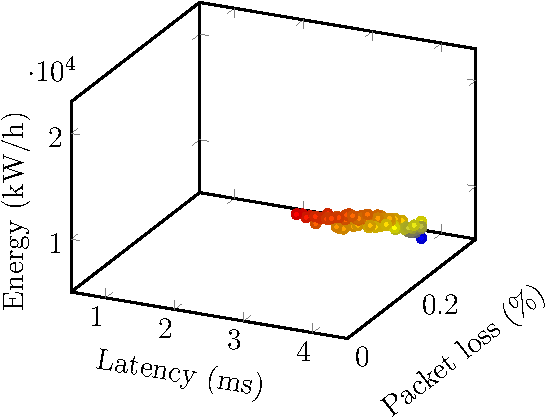
\includegraphics[width=\textwidth]{graphs/model/resources_energy-crop}
%         \caption{RU}
%     \end{subfigure}
%     \begin{subfigure}[b]{0.16\linewidth}
%         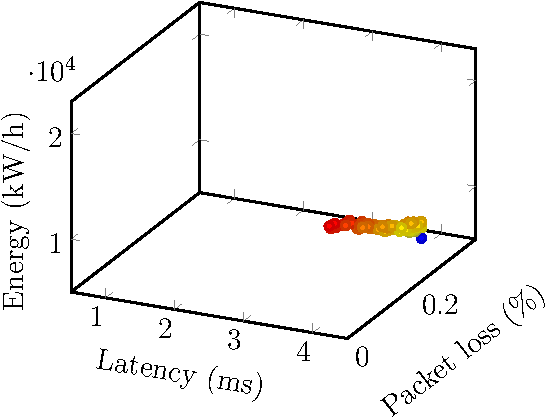
\includegraphics[width=\textwidth]{graphs/model/length_used-crop}
%         \caption{PLUS}
%     \end{subfigure}
%     \vspace{1em}
%     \caption{\textcolor{red}{Non-dominated front found by our algorithm when different models are used as the objective function.}}
%     \label{fig:model_objectives}
% \end{figure*}


\begin{figure}[t!]
    \centering
    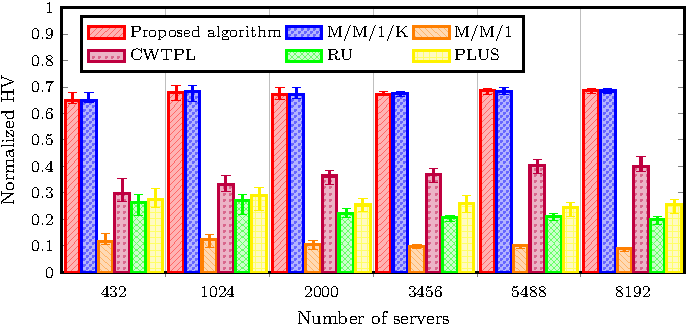
\includegraphics[width=\columnwidth]{graphs/model/models-crop}
    \caption{Inter-quartile range of the HV when using different surrogate models as the objective function.}
    \label{fig:model_benefits}
\end{figure}

\vspace{0.5em}
\noindent
\framebox{\parbox{\dimexpr\linewidth-2\fboxsep-2\fboxrule}{
        \textbf{\underline{Response to RQ3:}} \textit{The queueing models that account for the packet loss lead to significantly more diverse solutions compared to the other queueing model(s) as well as the surrogate models.}
    }}
\textcolor{red}{
\subsection{Evaluation of Solution Representation}
\label{sec:alternative_representations}
}
\textcolor{red}{To answer RQ4, we compare the quality of solutions obtained when different solution representations are applied to the VNFPP. Specifically, the following two meta-heuristic algorithms use NSGA-II as the baseline but have different solution representations.
\begin{itemize}
    \item\underline{Binary representation}: As in \cite{ChantreF20,KaurGK020,CharismiadisTPM20}, a string of binary digits are used to represent if a VNF is assigned to a server.
    \item\underline{Direct representation}: As in \cite{RankothgeLRL17}, a solution is directly represented as a string of VNFs.
\end{itemize}
In our experiments, we generate $30$ VNFPP instances for six data centers with different sizes. To compare the performance of different algorithms, we use the QoS model developed in~\pref{sec:system_model} to evaluate the objective functions of the solutions obtained by different algorithms and use the HV indicator as the performance measure.}

\begin{figure}[t!]
    \centering

    \begin{subfigure}[b]{0.48\linewidth}
        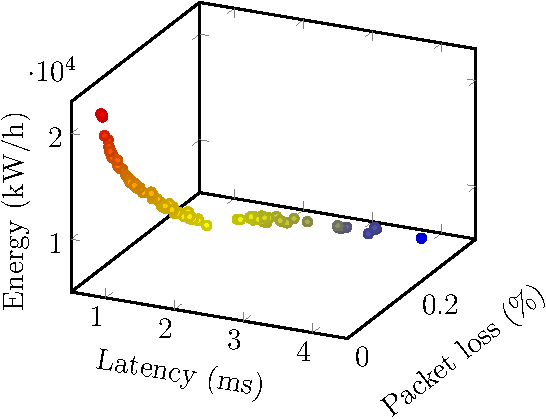
\includegraphics[width=\textwidth]{graphs/model/proposed-crop}
        \caption{Proposed}
    \end{subfigure}
    \begin{subfigure}[b]{0.48\linewidth}
        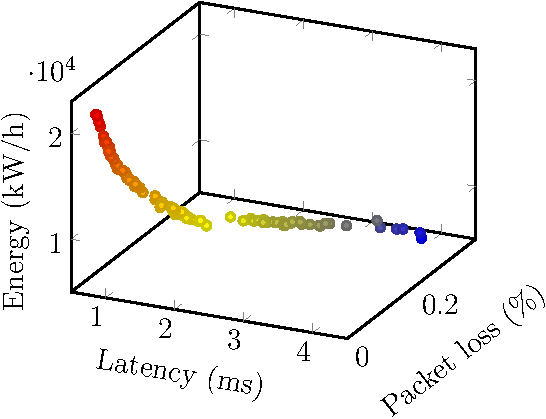
\includegraphics[width=\textwidth]{graphs/model/mm1k-crop}
        \caption{M/M/1/$B_c$}
    \end{subfigure}

    \vspace{1em}

    \begin{subfigure}[b]{0.48\linewidth}
        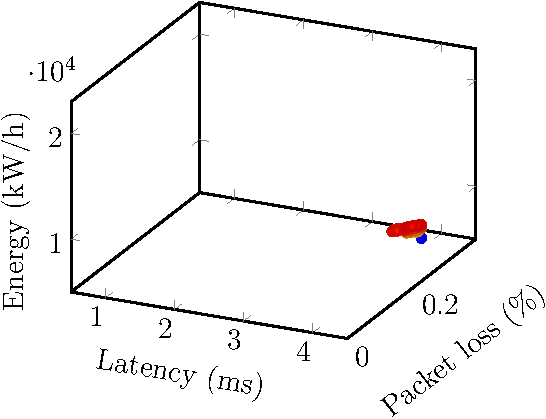
\includegraphics[width=\textwidth]{graphs/model/mm1-crop}
        \caption{M/M/1}
    \end{subfigure}
    \begin{subfigure}[b]{0.48\linewidth}
        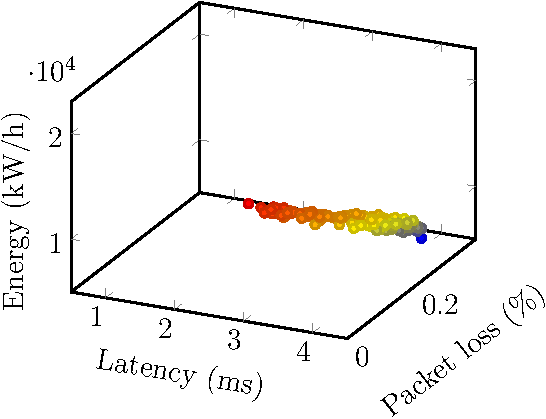
\includegraphics[width=\textwidth]{graphs/model/constant_energy-crop}
        \caption{CWTPL}
    \end{subfigure}

    \vspace{1em}

    \begin{subfigure}[b]{0.48\linewidth}
        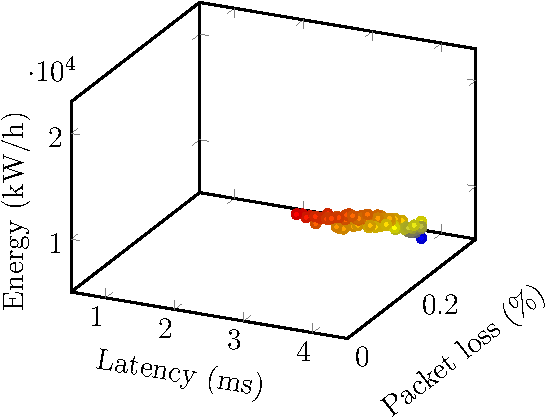
\includegraphics[width=\textwidth]{graphs/model/resources_energy-crop}
        \caption{RU}
    \end{subfigure}
    \begin{subfigure}[b]{0.48\linewidth}
        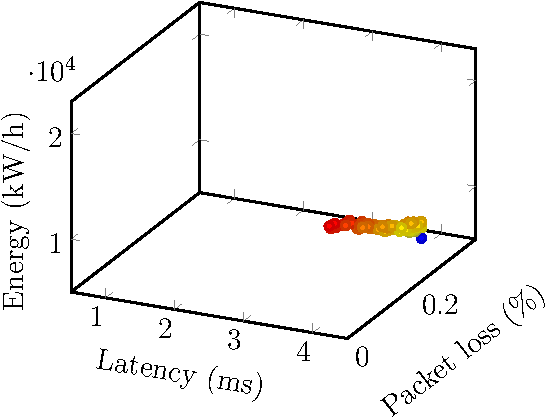
\includegraphics[width=\textwidth]{graphs/model/length_used-crop}
        \caption{PLUS}
    \end{subfigure}
    \vspace{1em}
    \caption{\textcolor{red}{Non-dominated front found by our algorithm when different models are used as the objective function.}}
    \label{fig:model_objectives}
\end{figure}

\begin{figure}[t!]
    \centering
    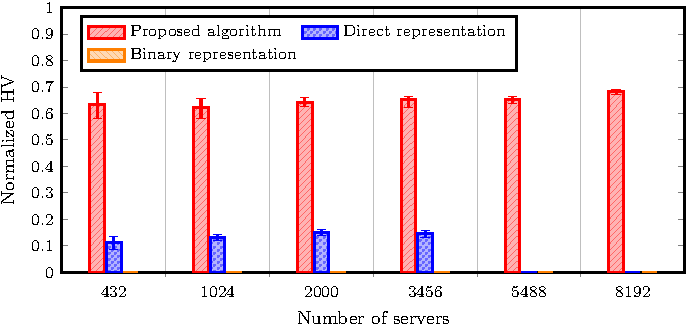
\includegraphics[width=\linewidth]{graphs/solution_representation/comparison-crop}
    \caption{Inter-quartile range of the HV when using different solution representations.}
    \label{fig:solution_representation_comparison}
\end{figure}
\begin{figure}[t!]
    \centering
    \begin{subfigure}[b]{0.49\linewidth}
        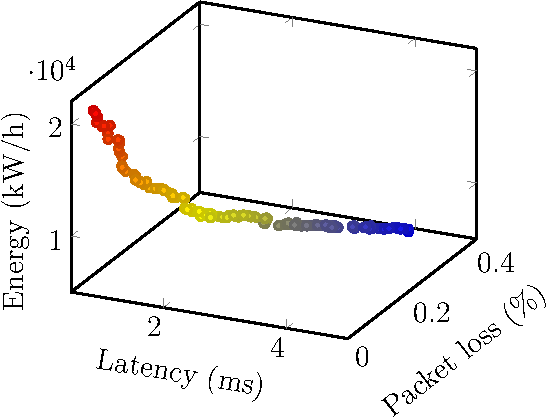
\includegraphics[width=\textwidth]{graphs/comparison/qm-crop}
        \caption{Proposed algorithm}
    \end{subfigure}
    \begin{subfigure}[b]{0.49\linewidth}
        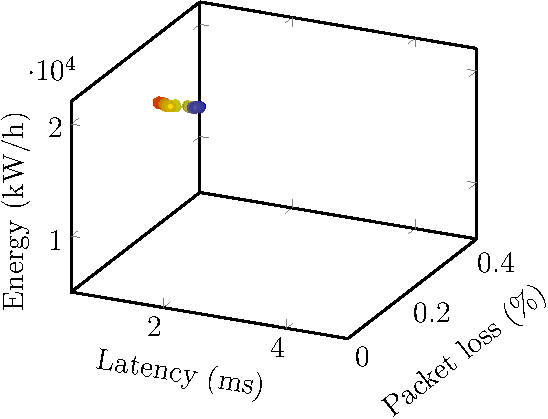
\includegraphics[width=\textwidth]{graphs/comparison/std-crop}
        \caption{Direct representation}
    \end{subfigure}

    \vspace{1em}
    \caption{Non-dominated front discovered when using different solution representations.}
    \label{fig:solution_representation_objectives}
\end{figure}

\textcolor{red}{
\subsubsection{Results}
From the results shown in Figs.~\ref{fig:solution_representation_comparison} and~\ref{fig:solution_representation_objectives}, we find that the solutions obtained by our proposed solution representation significantly outperform alternative representations. Our proposed solution representation has two advantages over existing representations. First, our proposed representation guarantees feasible solutions irregardless of the input. In contrast, both the direct and binary solution representations were unable to find feasible solutions to larger problem instances. Second, our proposed representation integrates domain knowledge to generate solutions with shorter average distances between VNFs causing the resultant solutions to be closer to the Pareto front than alternative representations. Existing solution representations do not utilize this information and instead rely solely on the optimization framework to locate high quality solutions.
}
\textcolor{red}{
Although the binary solution representation has been successfully applied to solve the VNFPP on small data centers (e.g.,~\cite{ChantreF20,KaurGK020,CharismiadisTPM20}), it does not scale well in the larger-scale problems considered in our experiments. With a binary solution representation, multiple VNFs to be placed on the same VM. This greatly complicates the search process compared to the direct or proposed solution representations with which this constraint is impossible to violate.
}
\textcolor{red}{
The direct solution representation is also only able to obtain feasible solutions to small data centers, as shown in~\pref{fig:solution_representation_objectives}, and exclusively finds solutions with high energy consumption. In particular, since a solution is only feasible when there is an instance of each VNF, solutions with more VNFs are more likely to be feasible than those with less VNFs and lower energy consumption. This leads the algorithm with the direct representation to be biased towards solutions with a high energy consumption. On larger problems with high numbers of VNFs, the direct solution representation is unable to find a solution with at least one instance of each VNF.
}

\vspace{0.5em}
\noindent
\framebox{\parbox{\dimexpr\linewidth-2\fboxsep-2\fboxrule}{
    \textcolor{red}{\textbf{\underline{Response to RQ4:}} \textit{The proposed solution representation allows the algorithm to discover significantly higher quality solutions than alternative solution representations.}}
    }}
    
\textcolor{red}{
\subsection{Comparison with Other Approaches}}
\label{sec:state_of_the_art}

\textcolor{red}{
\subsubsection{Methods}
To answer RQ5, we compare the performance of our tailored EMO algorithm with five state-of-the-art peer algorithms for solving VNFPPs. Specifically, the following two meta-heuristic algorithms use the NSGA-II as the baseline but use different genetic operators.
\begin{itemize}
    \item\underline{Binary representation}: In \cite{ChantreF20}, a string of binary digits are used to represent the placement of primary and secondary VNFs. To implement a fair comparison, we only consider the placement of the primary VNFs.
    \item\underline{Previous work}: We also compare our algorithm against our earlier work on this topic \cite{BillingsleyLMMG19}. This work utilized a direct representation with an earlier form of the tailored initialization operator.
\end{itemize}
The three heuristic algorithms are as follows.
\begin{itemize}
    \item\underline{BFDSU}~\cite{ZhangXLLGW17}: This is a modified best-fit decreasing heuristic that considers each VNF in turn and selects a server that can accommodate the VNF according to a predefined probability. In addition, the result is weighted towards selecting a server with a lower capacity.
    \item\underline{ESP-VDCE}~\cite{KaurGK020}: This is specifically designed for the Fat Tree data centers. It use a best fit approach but exclusively considers the servers nearest to where other VNFs of the same service have been placed.
    \item\underline{Stringer}~\cite{ChuaWZSH16}: This is also designed specifically for the Fat Tree data centers and it uses a round-robin placement strategy to place each VNF of each service in a sequence. The heuristic limits the available resources of each service and places a VNF on the first server with a sufficient capacity. If there is insufficient capacity in the data center for a VNF, the resources of each server are increased and the heuristic restarts from the first server.
\end{itemize}
Note that these heuristics assume that the number of service instances is known \textit{a priori}. Since each heuristic can only obtain a single solution, we generate a set of subproblems, each of which has a different number of service instances and is independently solved by a heuristic, to obtain a population of solutions at the end. In particular, we use the following two strategies to generate subproblems in our experiments.
\begin{itemize}
    \item One is to use the initialization operator developed in~\pref{sec:custom_operators} to serve our purpose. For the $i$th subproblem, the number of instances of the service $s$ is calculated as $N^I_{i,s}$ in~\pref{eq:num_services}.
    \item The other is to use the population obtained by our tailored EMO algorithm as a reference. For the $i$th subproblem, the number of instances of each service is the same as the $i$th solution obtained by our tailored EMO algorithm.
\end{itemize}
In our experiments, we generate $30$ VNFPP instances for six data centers with different sizes. To compare the performance of different algorithms, we use the QoS model developed in~\pref{sec:system_model} to evaluate the objective functions of the solutions obtained by different algorithms and use the HV indicator as the performance measure.
}
\textcolor{red}{
\subsubsection{Results}
}

\begin{figure*}[t!]
    \centering
    \begin{subfigure}[b]{0.19\linewidth}
        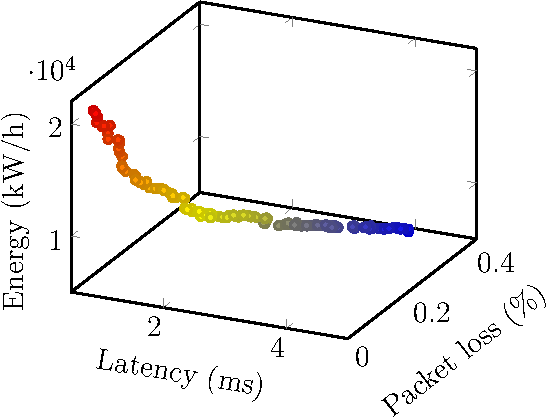
\includegraphics[width=\textwidth]{graphs/comparison/qm-crop}
        \caption{Proposed algorithm}
    \end{subfigure}
    \begin{subfigure}[b]{0.19\linewidth}
        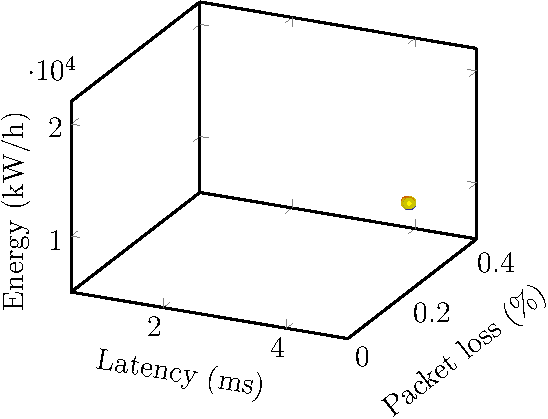
\includegraphics[width=\textwidth]{graphs/comparison/previous-crop}
        \caption{Previous algorithm}
    \end{subfigure}
    \begin{subfigure}[b]{0.19\linewidth}
        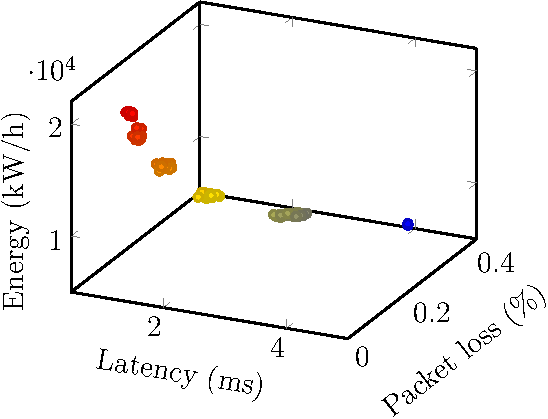
\includegraphics[width=\textwidth]{graphs/comparison/esp_vdce-crop}
        \caption{ESP-VDCE \cite{KaurGK020}}
    \end{subfigure}
    \begin{subfigure}[b]{0.19\linewidth}
        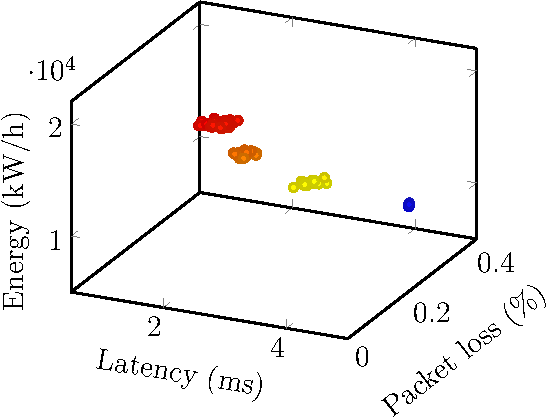
\includegraphics[width=\textwidth]{graphs/comparison/bfdsu-crop}
        \caption{BFDSU \cite{ZhangXLLGW17}}
    \end{subfigure}
    \begin{subfigure}[b]{0.19\linewidth}
        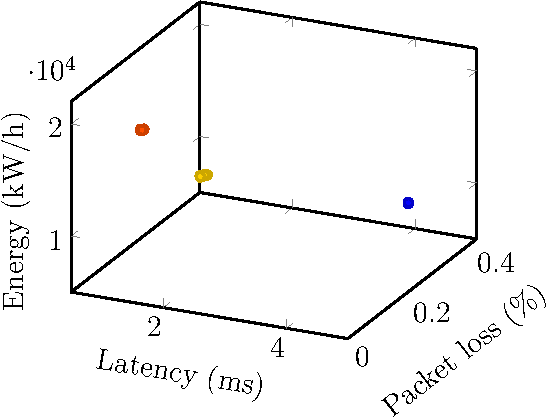
\includegraphics[width=\textwidth]{graphs/comparison/stringer-crop}
        \caption{Stringer \cite{ChuaWZSH16}}
    \end{subfigure}

    \vspace{1em}
    \caption{Non-dominated front found by five algorithms. Subproblems for the heuristic algorithms were generated using our proposed initialization operator. The binary solution representation is omitted as it resulted in no feasible solution at all.}
    \label{fig:alg_objectives}
\end{figure*}

\begin{figure*}
    \centering
    \hfill
    \begin{minipage}[t]{.48\textwidth}
        \centering
        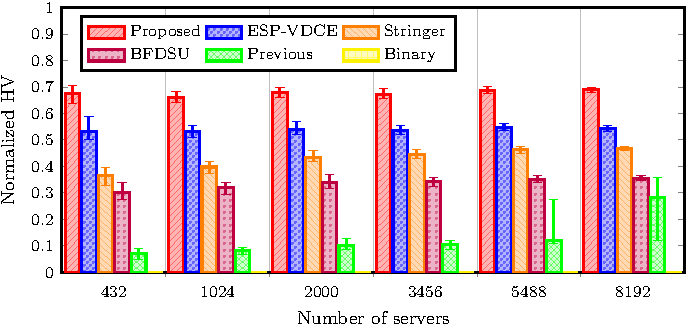
\includegraphics[width=\columnwidth]{graphs/comparison/comparison-crop}
        \caption{Inter-quartile range of the HV when using the initialization operator to generate subproblems for the heuristic algorithms.}
        \label{fig:alg_comparison}
    \end{minipage}\hfill
    \begin{minipage}[t]{.48\textwidth}
        \centering
        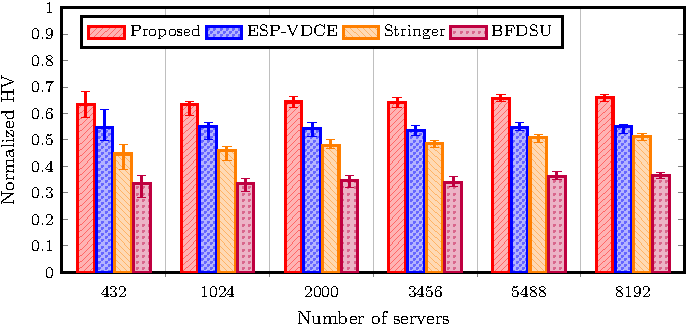
\includegraphics[width=\columnwidth]{graphs/comparison/alg_fixed-crop}
        \caption{Inter-quartile range of the HV when using the solutions of our proposed algorithm to generate subproblems for the heuristic algorithms.}
        \label{fig:alg_fixed}
    \end{minipage}
    \hfill
\end{figure*}

\textcolor{red}{
From the results shown in~\pref{fig:alg_comparison} and~\pref{fig:alg_fixed}, it is clear that our proposed algorithm outperforms other competitors on all test cases. This can be attributed to our two proposed operators. First, it is clear from \pref{fig:alg_objectives} that proposed operators enable a diverse population of solutions. Our two proposed operators work together towards this goal. The initialization operator produces a diverse range of possible solutions, whilst the solution representation ensures that these solutions are feasible.
}

\textcolor{red}{
Second, our proposed solution representation minimizes the distance between sequential VNFs, improving the overall QoS. We note that the two best performing algorithms, our proposed algorithm and ESP-VDCE, aim to minimize the distance between sequential VNFs. In contrast, both BFDSU and Stringer tend to produce longer path lengths thus lead to significantly worse solutions than our proposed algorithm. Since Stringer restricts the capacity of each server, it causes services to be placed across multiple servers. Likewise, the stochastic component of BFDSU can cause it to place VNFs far away from any other VNF of the service. In contrast, our proposed algorithm incorporates useful information into the optimization process and places sequential VNFs close by thus leading to better solutions.
}

\textcolor{red}{
A final benefit of our algorithm is that it can iteratively improve the placements to minimize the energy consumption and QoS. Although ESP-VDCE does consider the path length, it otherwise uses a simple first fit heuristic that cannot consider how service instances should be placed in relation to each other. As a consequence, the performance of ESP-VDCE depends on the order in which services are considered. Our proposed algorithm considers the problem holistically and can make informed placement decisions.
}

\vspace{1em}
\noindent
\framebox{\parbox{\dimexpr\linewidth-2\fboxsep-2\fboxrule}{
        \textcolor{red}{\textbf{\underline{Response to RQ5:}} \textit{Our proposed tailored EMO algorithm obtains significantly better solutions in terms of both convergence and diversity compared to other state-of-the-art peer algorithms.}}
    }}

\subsection{Effectiveness on Constraint Handling}
\label{sec:custom_operators}

\subsubsection{Methods}

RQ6 aims to validate the effectiveness of our proposed solution representation for handling challenging anti-affinity and limited licenses constraints. We generated $30$ problem instances for a small data center with $412$ servers\footnote{Only the small data center is considered here in view of the poor scalability of the direct representation reported in~\pref{sec:state_of_the_art}.}. Note that we only compare our proposed algorithm with the meta-heuristic approach with the direct solution representation in our experiments given the poor performance of the binary solution representation reported in~\pref{sec:state_of_the_art} and the inability of the heuristic approaches to solve constrained VNFPPs.

For the anti-affinity constraints, we considered different numbers of anti-affinity services and similarly, for the limited licenses constraints we considered different numbers of limited license VNFs and different numbers of licenses for each VNF. Since different VNFs have different service rates, we calculate the expected maximum number of instances of each VNF that could be accommodated by the data center (i.e. the maximum value of $N^I$ in the \pref{eq:num_services}) and restrict the solution to use a fraction of this number of licenses.

\subsubsection{Results}
From the results shown in Figs.~\ref{fig:anti_affinity} and \ref{fig:limited_licenses}, it is clear to see that the direct representation cannot find any feasible solution due to the narrow feasible search space. In contrast, our proposed operators are still able to find a diverse set of feasible solutions even for these highly constrained problems. As shown in \pref{fig:anti_affinity}, our algorithm produces consistently good results on the anti-affinity problems. This is a benefit of our proposed solution representation which ensures the satisfaction of the anti-affinity constraints. Since the solutions are guaranteed to be feasible, the algorithm should only optimize the number and placement of service instances. Any degradation in the HV indicator can be attributed to the narrower feasible search space causing better alternatives to be infeasible. In particular, anti-affinity constraints prevent VNFs of other services from being placed on a server thus can prevents a server from being fully utilized.

According to our empirical results, the limited licenses constraints appear to be more challenging. As shown in~\pref{fig:limited_licenses}, populations obtained by our proposed algorithm have a better HV value when a large number of licenses is allowed, whereas it falls down when fewer licenses are available. Furthermore, the percentage of VNFs that are affected has little impact. The lower HV values can be explained by a loss of diversity as a result of the feasible solution space being constrained. If any VNF in a service is constrained by a limited license constraint, this limits the number of service instances that can be placed. Hence the percentage of VNFs that can be placed is less significant as it is likely that a VNF in the service is already constrained.

\vspace{1em}
\noindent
\framebox{\parbox{\dimexpr\linewidth-2\fboxsep-2\fboxrule}{
        \textbf{\underline{Response to RQ6:}} \textit{From our empirical results, we find that our proposed genotype-phenotype solution representation is superior for handling highly constrained VNFPP.}
    }}

\begin{figure}[t!]
    \centering
    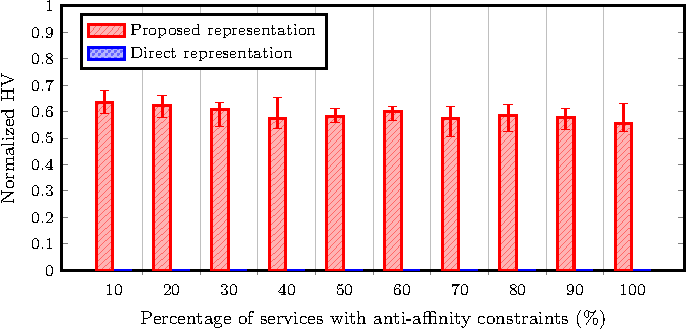
\includegraphics[width=\linewidth]{graphs/constraints/anti_affinity-crop}
    \caption{Inter-quartile range of the HV for different solution representations and anti-affinity constraints.}
    \label{fig:anti_affinity}
\end{figure}
\begin{figure}[t!]
    \centering
    \begin{subfigure}[b]{0.48\linewidth}
        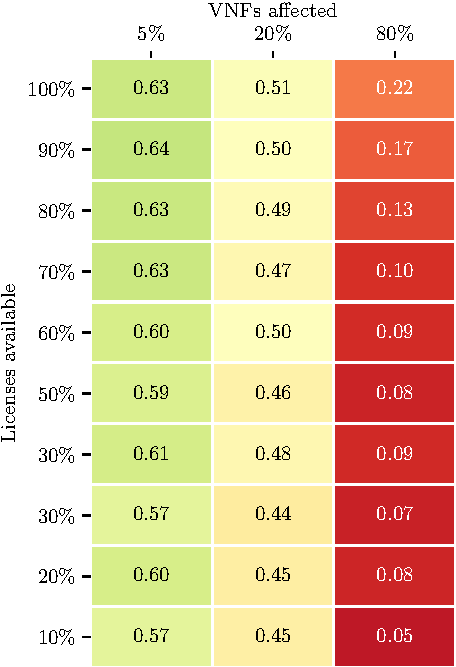
\includegraphics[width=\textwidth]{graphs/constraints/ca_NSGAII_LIM-crop}
        \caption{Proposed representation}
    \end{subfigure}
    \vspace{1em}
    \begin{subfigure}[b]{0.3732\linewidth}
        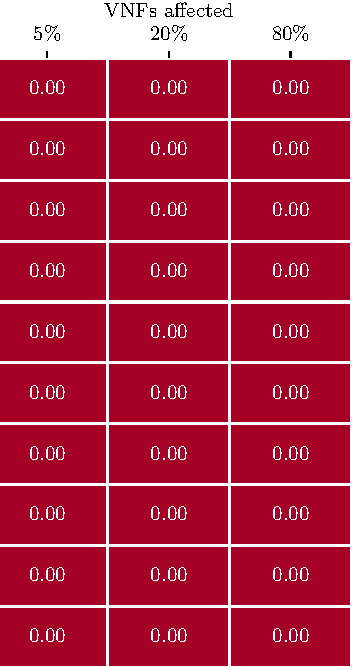
\includegraphics[width=\textwidth]{graphs/constraints/std_NSGAII_LIM-crop}
        \caption{Direct representation}
    \end{subfigure}
    \vspace{0.3em}

    \hspace{2em}
    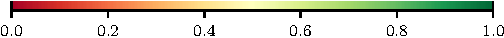
\includegraphics[width=.8\linewidth]{graphs/constraints/key-crop}
    \caption{Mean normalized HV under max license constraints.}
    \label{fig:limited_licenses}
\end{figure}
